\section{问题一:确定性环境下的多周期优化模型}

问题一旨在为该乡村规划2024年至2030年共七年的农作物种植策略。从微观经济学视角看,这相当于将该乡村抽象为一个理性的经济主体,其在拥有固定的生产技术、资源和已知的市场参数条件下,追求长期利润的最大化。由于决策变量中既包含连续的种植面积,也包含是否种植的离散选择,该问题能够被构建为一个大规模的多周期混合整数线性规划(MILP)模型。本章将详细阐述该模型的构建、求解与分析过程,旨在为后续更复杂的分析提供一个确定性条件下的最优基准。

模型的顶层设计如图\ref{fig:milp_framework}所示,它展示了模型的输入、处理核心与输出。该框架整合了土地资源、作物属性、经济参数和农艺规则,通过MILP求解器进行优化,最终生成最优的七年种植方案与相应的经济效益预测。

\begin{figure}[htbp]
    \centering
    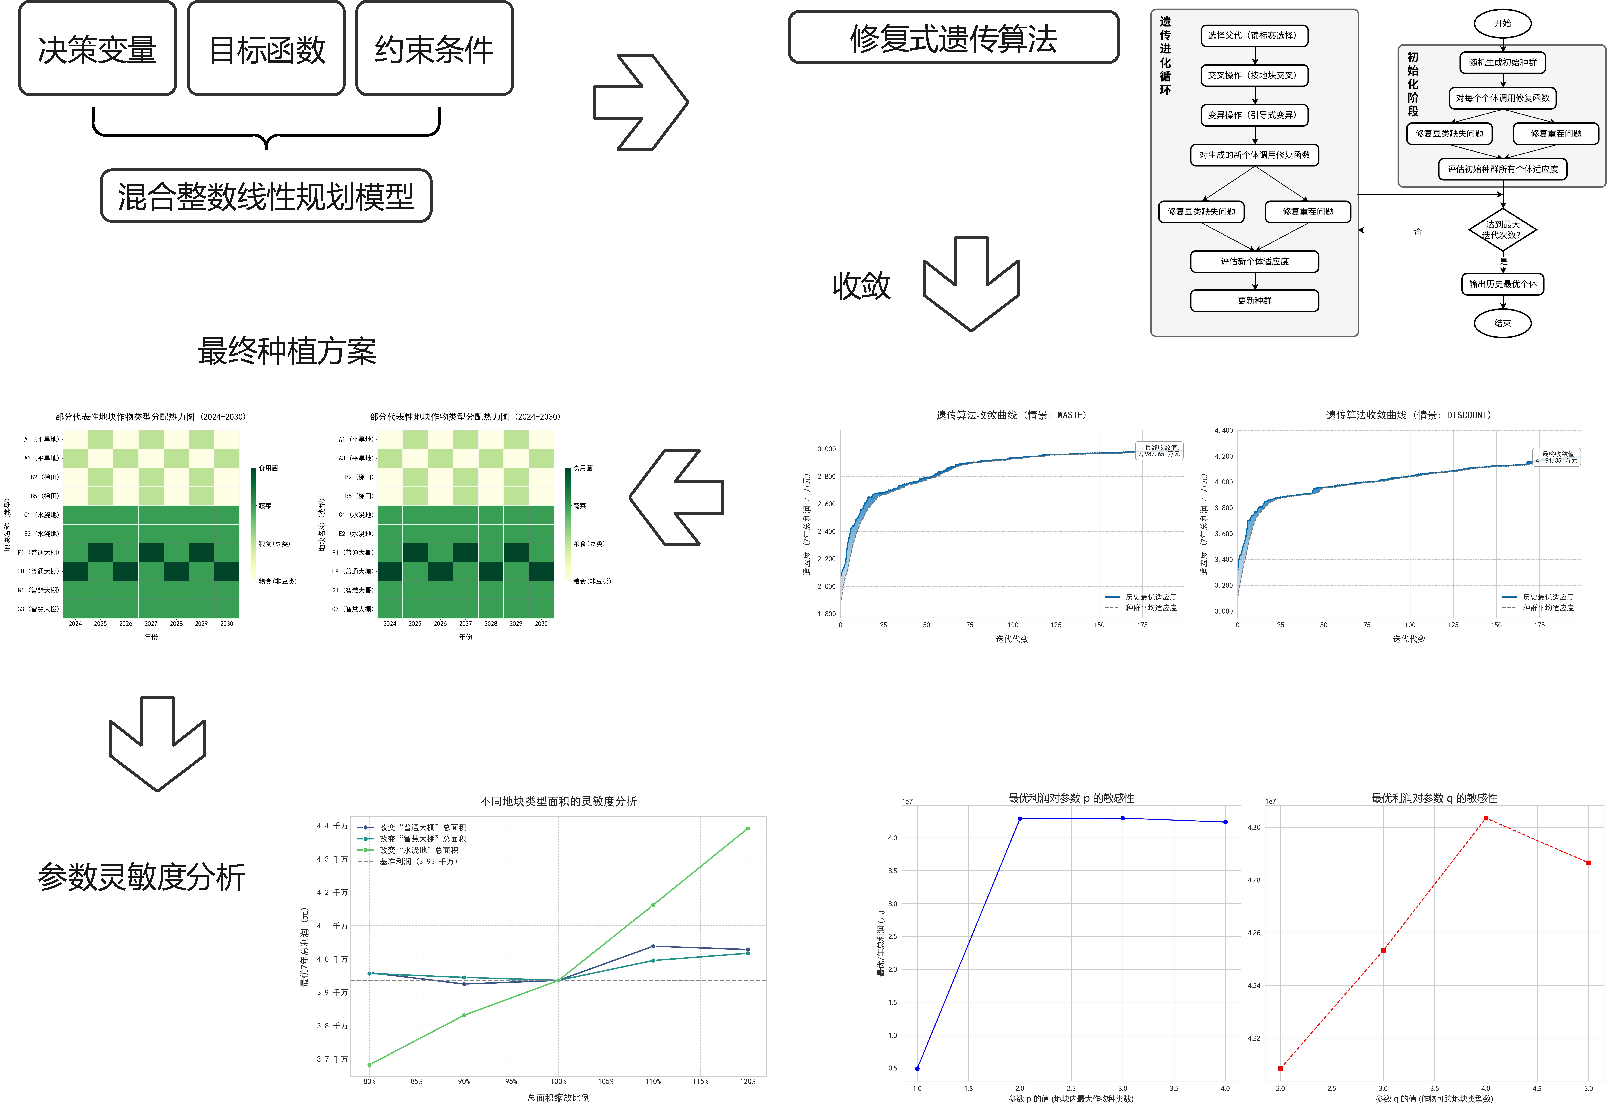
\includegraphics[width=0.8\textwidth]{figs/3问题一/问题一框架.pdf}
    \caption{问题一的混合整数线性规划模型概念框架图。}
    \label{fig:milp_framework}
\end{figure}

\subsection{模型构建}


为将该乡村的长期种植规划问题转化为一个可求解的数学模型,我们构建了一个多周期混合整数线性规划(MILP)模型。该模型以古典微观经济学中的厂商理论为基础,将乡村视为一个追求长期利润最大化的理性决策主体。模型的构建过程遵循模块化原则,依次定义了决策变量、目标函数和约束条件三个核心部分。

\subsubsection{决策变量}

模型的决策核心在于如何在给定的时间和空间维度上分配种植资源。为此,我们定义了以下四组核心决策变量,它们共同构成了完整的七年种植方案:
\begin{itemize}
    \item $a_{ijky}$: 一个连续变量,表示在年份 $y$ 的第 $k$ 季,于地块 $i$ 上种植作物 $j$ 的面积(亩)。
    \item $x_{ijky}$: 一个二进制变量,当 $a_{ijky} > 0$ 时为1,否则为0。它表示是否在年份 $y$ 的第 $k$ 季,于地块 $i$ 上安排种植作物 $j$。
    \item $\text{normal}_{jy}$: 一个连续辅助变量,表示年份 $y$ 作物 $j$ 未超出预期销售量的产量部分(斤)。
    \item $\text{over}_{jy}$: 一个连续辅助变量,表示年份 $y$ 作物 $j$ 超出预期销售量的产量部分(斤)。
\end{itemize}



\subsubsection{目标函数}

模型的总体目标是最大化2024年至2030年这七年间的累计总利润。总利润定义为总销售收入与总种植成本的差额。总种植成本的计算公式为:
\begin{equation}
\text{Cost} = \sum_{y \in Y} \sum_{i \in I} \sum_{j \in J} \sum_{k \in K} a_{ijky} \cdot C_{jy}
\end{equation}
根据题目要求,针对超出预期销售量的农产品处置方式,分别构建了两种情景下的目标函数。

\textbf{情景 1:超出部分滞销}

在此情景下,任何超出预期销售量的产品均无市场价值,总收入仅来源于正常销售部分。因此,目标函数 $Z_1$ 定义为:
\begin{equation}
\text{Maximize} \quad Z_1 = \sum_{y \in Y} \sum_{j \in J} (\text{normal}_{jy} \cdot P_{jy}) - \text{Cost}
\end{equation}

\textbf{情景 2:超出部分降价出售}

在此情景下,超出预期销售量的产品可以按正常价格的50\%进行销售,从而产生额外收入。因此,目标函数 $Z_2$ 定义为:
\begin{equation}
\text{Maximize} \quad Z_2 = \sum_{y \in Y} \sum_{j \in J} (\text{normal}_{jy} \cdot P_{jy} + \text{over}_{jy} \cdot (0.5 \cdot P_{jy})) - \text{Cost}
\end{equation}

\subsubsection{约束条件}

为确保种植方案在现实中可实施、在农艺上合理、在生态上可持续,我们建立了系统的约束集。该约束覆盖土地、劳动力、用水与设施容量等物理资源上限。包含种植制度、轮作间隔与病虫害防控等农艺要求。纳入产销平衡、价格与合同约束、库存与流通能力等市场规则。加入土壤养分恢复、水资源红线与排放限额等长期生态限制。上述约束以可检验的数学形式(线性不等式与逻辑条件)进入模型,并在求解过程中严格满足。

\textbf{1. 总产量与销售部分关联}

为建立生产与市场销售之间的平衡关系,任何一种作物的年总产量必须等于其正常销售量与超预期销售量之和。同时,其正常销售部分的产量不能突破市场的预期销售量上限。
\begin{gather}
\sum_{i \in I} \sum_{k \in K} a_{ijky} \cdot \text{yield}_{jy} = \text{normal}_{jy} + \text{over}_{jy} \quad (\forall j \in J, y \in Y) \label{eq:yield_balance} \\
\text{normal}_{jy} \le \text{sale}_{jy} \quad (\forall j \in J, y \in Y) \label{eq:normal_sale_limit}
\end{gather}
此外,所有与面积和产量相关的变量均需满足非负性。
\begin{equation}
a_{ijky}, \text{normal}_{jy}, \text{over}_{jy} \ge 0 \label{eq:non_negativity}
\end{equation}

\textbf{2. 决策变量关联}

为确保二进制决策变量 $x_{ijky}$ 与连续决策变量 $a_{ijky}$ 的逻辑一致性,即仅当决定进行某项种植活动时 ($x_{ijky}=1$),相应的种植面积 ($a_{ijky}$) 才可为正,引入以下约束。其中,$M$ 是一个足够大的正数,$\epsilon$ 是一个极小的正数,用以规定最小种植阈值。
\begin{gather}
a_{ijky} \le M \cdot x_{ijky} \quad (\forall i, j, k, y) \label{eq:big_m} \\
a_{ijky} \ge \epsilon \cdot x_{ijky} \quad (\forall i, j, k, y) \label{eq:min_area}
\end{gather}

\textbf{3. 土地适宜性约束}

农作物的生长对其环境有特定要求,因此任何种植安排都必须遵循农作物对土地类型和季节的适应性。
\begin{equation}
x_{ijky} \le S_{ijk} \quad (\forall i, j, k, y) \label{eq:suitability}
\end{equation}

\textbf{4. 地块面积约束}

任何地块在任一季节内,所有作物的种植面积之和不能超过该地块的物理总面积。
\begin{equation}
\sum_{j \in J} a_{ijky} \le A_i \quad (\forall i \in I, k \in K, y \in Y) \label{eq:area_limit}
\end{equation}

\textbf{5. 重茬约束}

为了维护土壤健康和防止产量下降,模型禁止在同一地块连续两年种植同一种作物。该农艺规则通过引入辅助二进制变量 $z_{ijy}$ 来实现,该变量用以标记作物 $j$ 在年份 $y$ 是否在地块 $i$ 上种植过。
\begin{gather}
z_{ijy} \ge x_{ijky} \quad (\forall i, j, k, y) \label{eq:z_def1} \\
\sum_{k \in K} x_{ijky} \ge z_{ijy} \quad (\forall i, j, y) \label{eq:z_def2} \\
z_{ijy} + z_{ij,y-1} \le 1 \quad (\forall i, j, y) \label{eq:rotation}
\end{gather}
对于规划的起始年份2024年,此约束需与2023年的种植历史数据 $H_{ij,2023}$ 进行衔接。
\begin{equation}
z_{ij,2024} + H_{ij,2023} \le 1 \quad (\forall i, j) \label{eq:rotation_init}
\end{equation}

\textbf{6. 豆类种植约束}

基于豆类作物能够固氮改良土壤的特性,规定所有地块在任意连续三年周期内,必须至少安排一次豆类作物的种植。
\begin{equation}
\sum_{j \in J_{\text{legume}}} (z_{ij,y} + z_{ij,y+1} + z_{ij,y+2}) \ge 1 \quad (\forall i, y \in \{2024, \dots, 2028\}) \label{eq:legume}
\end{equation}
此约束的初始条件也需要结合2022年和2023年的历史种植数据进行调整,以保证规则的完整性。

\textbf{7. 分散性约束}

为提高耕作效率和方便田间管理,对种植方案的作物分布施加限制。首先,在同一季节,每个地块内种植的作物种类不应超过预设上限 $p$。
\begin{equation}
\sum_{j \in J} x_{ijky} \le p \quad (\forall i, k, y) \label{eq:p_limit}
\end{equation}
其次,为避免单一作物过于分散地种植,规定在同一季节,每种作物允许种植的地块类型数量不应超过预设上限 $q$。此约束通过引入辅助二进制变量 $w_{jtky}$ 实现,该变量标记作物 $j$ 是否在年份 $y$ 的 $k$ 季种植于类型为 $t$ 的土地上。
\begin{gather}
x_{ijky} \le w_{jtky} \quad \text{where } t = \text{Type}(i) \quad (\forall i, j, k, y) \label{eq:w_def1} \\
\sum_{i \in I, \text{Type}(i)=t} x_{ijky} \ge w_{jtky} \quad (\forall j, t, k, y) \label{eq:w_def2} \\
\sum_{t \in T} w_{jtky} \le q \quad (\forall j, k, y) \label{eq:q_limit}
\end{gather}







\subsubsection{优化模型的整合呈现}

基于前文对各组成要素的定义,现给出混合整数线性规划模型的完整表述。该表述包含决策变量、目标函数,以及关于市场、土地、农艺与管理的全部约束。由此形成用于求解最优种植方案的数学框架。模型的总目标为最大化总利润$Z$。针对题目中超售产品处置的两种情景,$Z$的计算公式分别定义如下:
\begin{itemize}
    \item \textbf{情景 1 (滞销):} $Z = \sum_{y \in Y} \sum_{j \in J} (\text{normal}_{jy} \cdot P_{jy}) - \text{Cost}$
    \item \textbf{情景 2 (降价出售):} $Z = \sum_{y \in Y} \sum_{j \in J} (\text{normal}_{jy} \cdot P_{jy} + \text{over}_{jy} \cdot (0.5 \cdot P_{jy})) - \text{Cost}$
\end{itemize}
其中,总成本 $\text{Cost} = \sum_{y \in Y} \sum_{i \in I} \sum_{j \in J} \sum_{k \in K} a_{ijky} \cdot C_{jy}$。

完整的优化模型表述为:
\begin{flalign}
    \text{Maximize} \quad & Z & \\
    \text{subject to} \quad & \sum_{i \in I} \sum_{k \in K} a_{ijky} \cdot \text{yield}_{jy} = \text{normal}_{jy} + \text{over}_{jy} & \forall j, y \label{con:yield_balance} \\
    & \text{normal}_{jy} \le \text{sale}_{jy} & \forall j, y \label{con:normal_sale_limit} \\
    & a_{ijky} \le M \cdot x_{ijky} & \forall i, j, k, y \label{con:big_m} \\
    & a_{ijky} \ge \epsilon \cdot x_{ijky} & \forall i, j, k, y \label{con:min_area} \\
    & x_{ijky} \le S_{ijk} & \forall i, j, k, y \label{con:suitability} \\
    & \sum_{j \in J} a_{ijky} \le A_i & \forall i, k, y \label{con:area_limit} \\
    & z_{ijy} \ge x_{ijky} & \forall i, j, k, y \label{con:z_def1} \\
    & \sum_{k \in K} x_{ijky} \ge z_{ijy} & \forall i, j, y \label{con:z_def2} \\
    & z_{ijy} + z_{ij,y-1} \le 1 & \forall i, j, y \label{con:rotation} \\
    & z_{ij,2024} + H_{ij,2023} \le 1 & \forall i, j \label{con:rotation_init} \\
    & \sum_{j \in J_{\text{legume}}} (z_{ij,y} + z_{ij,y+1} + z_{ij,y+2}) \ge 1 & \forall i, y \in \{2024, \dots, 2028\} \label{con:legume} \\
    & \sum_{j \in J} x_{ijky} \le p & \forall i, k, y \label{con:p_limit} \\
    & x_{ijky} \le w_{jtky}, \quad t = \text{Type}(i) & \forall i, j, k, y \label{con:w_def1} \\
    & \sum_{i \in I, \text{Type}(i)=t} x_{ijky} \ge w_{jtky} & \forall j, t, k, y \label{con:w_def2} \\
    & \sum_{t \in T} w_{jtky} \le q & \forall j, k, y \label{con:q_limit} \\
    & a_{ijky}, \text{normal}_{jy}, \text{over}_{jy} \ge 0 & \forall i, j, k, y \label{con:non_negativity} \\
    & x_{ijky}, z_{ijy}, w_{jtky} \in \{0, 1\} & \forall i, j, t, k, y \label{con:binary}
\end{flalign}


\subsection{模型求解与算法设计}

前文构建的混合整数线性规划模型,因其决策变量众多、约束条件复杂且相互交织,构成了一个典型的NP-Hard组合优化问题。该问题的解空间随着规划年限和地块数量的增加而呈指数级增长,导致传统的精确求解方法,如穷举搜索,在计算上是不可行的。尽管商业或开源的精确求解器(如CBC、Gurobi)理论上能够找到全局最优解,但在面对如此大规模的实例时,其求解时间往往难以接受,且建模过程相对繁琐。因此,为了在有限时间内获得高质量的可行解,本文设计并实现了一种启发式算法进行求解,其框架如图\ref{fig:algorithm_framework}所示。

\begin{figure}[htbp]
    \centering
    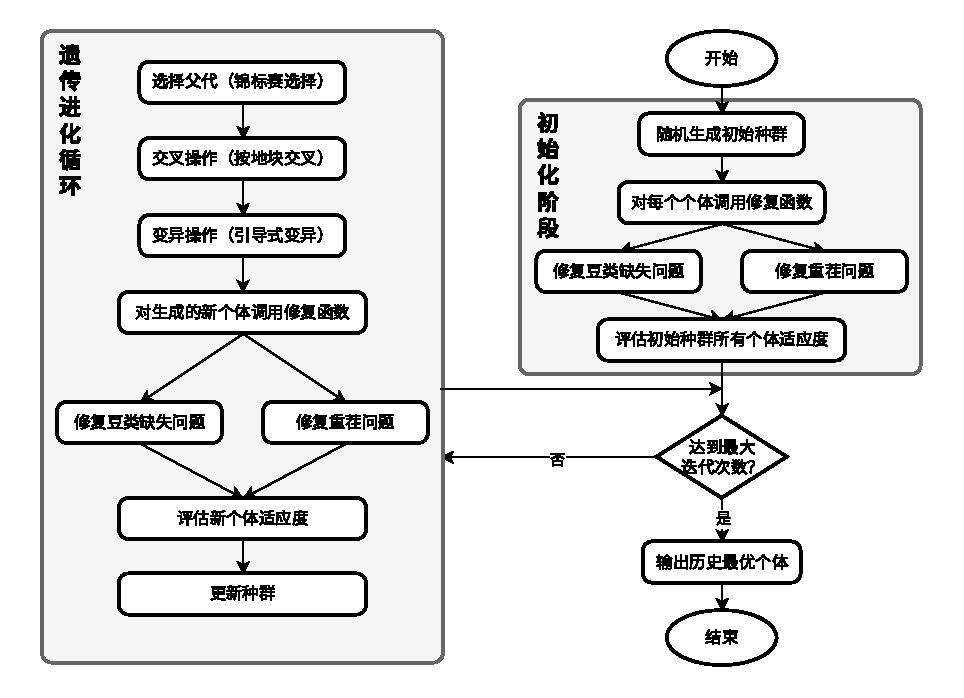
\includegraphics[width=0.9\textwidth]{figs/3问题一/遗传算法图.pdf}
    \caption{修复式遗传算法框架}
    \label{fig:algorithm_framework}
\end{figure}


\subsubsection{算法选择与基本原理}

在算法选型阶段,我们评估了多种方案。初步尝试的基础遗传算法依赖于惩罚函数来处理约束,但实践表明,由于本模型存在大量严格的“硬”约束(例如重茬和豆类轮作),随机生成的初始解几乎全部违反约束。这导致适应度函数被巨大的惩罚项主导,使得算法难以在广阔的不可行域中有效搜索,收敛性能不佳。

为了克服这一挑战,我们最终选择采用一种\textbf{修复式遗传算法}。该方法的核心思想是将领域知识,即模型的各项约束规则,内嵌到一个确定性的“修复函数”中。遗传算法强大的全局搜索能力得以保留,同时通过修复机制保证了在进化的每一个环节(包括种群初始化、交叉和变异之后),所有个体都始终是满足核心约束的可行解。这种设计将算法的搜索焦点从“如何避免违反约束”转移到“如何在可行域内寻找更优解”,从而显著净化了搜索空间,极大地提升了算法的收敛效率和稳定性。

\subsubsection{修复式遗传算法实现细节}

\textbf{解决方案编码}

为了直观地表示一个完整的七年种植计划,我们采用结构化的字典对染色体进行编码。其基本格式为:{年份: {季节: {地块名称: 作物名称}}}。例如,一个个体中的\text{solution[2025][1]['A1']} = '玉米',明确表示2025年第一季在A1地块种植玉米。此编码方式不仅便于理解,也为后续的遗传算子操作提供了便利。

\textbf{适应度函数}

适应度函数直接定义为问题所追求的七年总利润,其计算方式与目标函数一致。根据两种不同的市场情景(超出部分滞销或折价出售),我们实现了相应的收入计算逻辑。由于所有核心约束均由修复函数处理,适应度函数中不包含任何惩罚项,确保了其评估的纯粹性,即直接反映解的经济效益。

\textbf{修复函数}

修复函数是本算法的关键所在,它在种群初始化以及每次交叉和变异操作后被调用,以确保所有个体始终满足农艺要求。该函数主要执行两项修复任务:
\begin{itemize}
    \item 修复重茬问题:算法会遍历方案中的所有地块和年份,检查是否存在与前一年种植相同作物的情况。一旦发现重茬,系统将从一个预先定义的、不包含前一年作物的合法候选作物列表中,随机选择一种进行替换。
    \item 修复豆类缺失问题: 算法会遍历所有地块的每一个三年窗口期(起始于2023年)。若发现某个窗口期内未能满足至少种植一次豆类作物的要求,系统将强制在该窗口期内的某一年随机选择一个季节,将原定作物替换为一种合法的、且不与前一年构成重茬的豆类作物。
\end{itemize}

\textbf{遗传算子}

\begin{itemize}
    \item \textbf{选择:} 采用经典的锦标赛选择机制。每次从种群中随机选择$k$个个体(本文设$k=3$),并将其中适应度最高的个体选入下一代种群的父代池。
    \item \textbf{交叉:} 设计了按地块交叉的策略。以一定的交叉概率,随机选择若干地块,然后交换两个父代个体在这些选定地块上的完整七年种植历史,从而生成子代。
    \item \textbf{变异:} 采用引导式变异。随机选择方案中的若干基因位点(即某个地块在某年某季的种植决策),并从一个预先筛选好的、针对该地块和季节的“合法作物列表”中随机选择一种新作物进行替换。这种方式保证了变异操作本身不会引入明显不合理的种植安排。
\end{itemize}

\textbf{主要超参数设置}

通过多次调试与实验,我们为算法设定了一组表现良好的关键超参数,具体如下:种群大小为100,最大迭代代数为200,交叉概率为0.8,变异概率为0.2。


\subsection{求解结果与分析}

基于上述模型与算法,我们分别对情景一(超出部分滞销)和情景二(超出部分降价出售)进行了求解。本节将展示算法的收敛性能、最优种植方案的构成以及各类作物的具体产量安排。

\subsubsection{算法收敛性分析}


为了验证修复式遗传算法的有效性,我们追踪并记录了其在200次迭代过程中的适应度变化。如图\ref{fig:convergence}所示,横轴为进化代数,纵轴为七年总利润。图中展示了每一代种群的历史最优适应度与平均适应度。

在两种情景下,最优适应度曲线快速上升,并分别收敛于2987.65万元与4191.35万元。这表明算法能在有限迭代内找到高质量解。平均适应度曲线平稳增长。两条曲线在后期逐渐趋近,说明种群整体向最优解集中,形成稳定收敛。

\begin{figure}[H]
    \centering
    \begin{subfigure}[b]{0.48\textwidth}
        \centering
        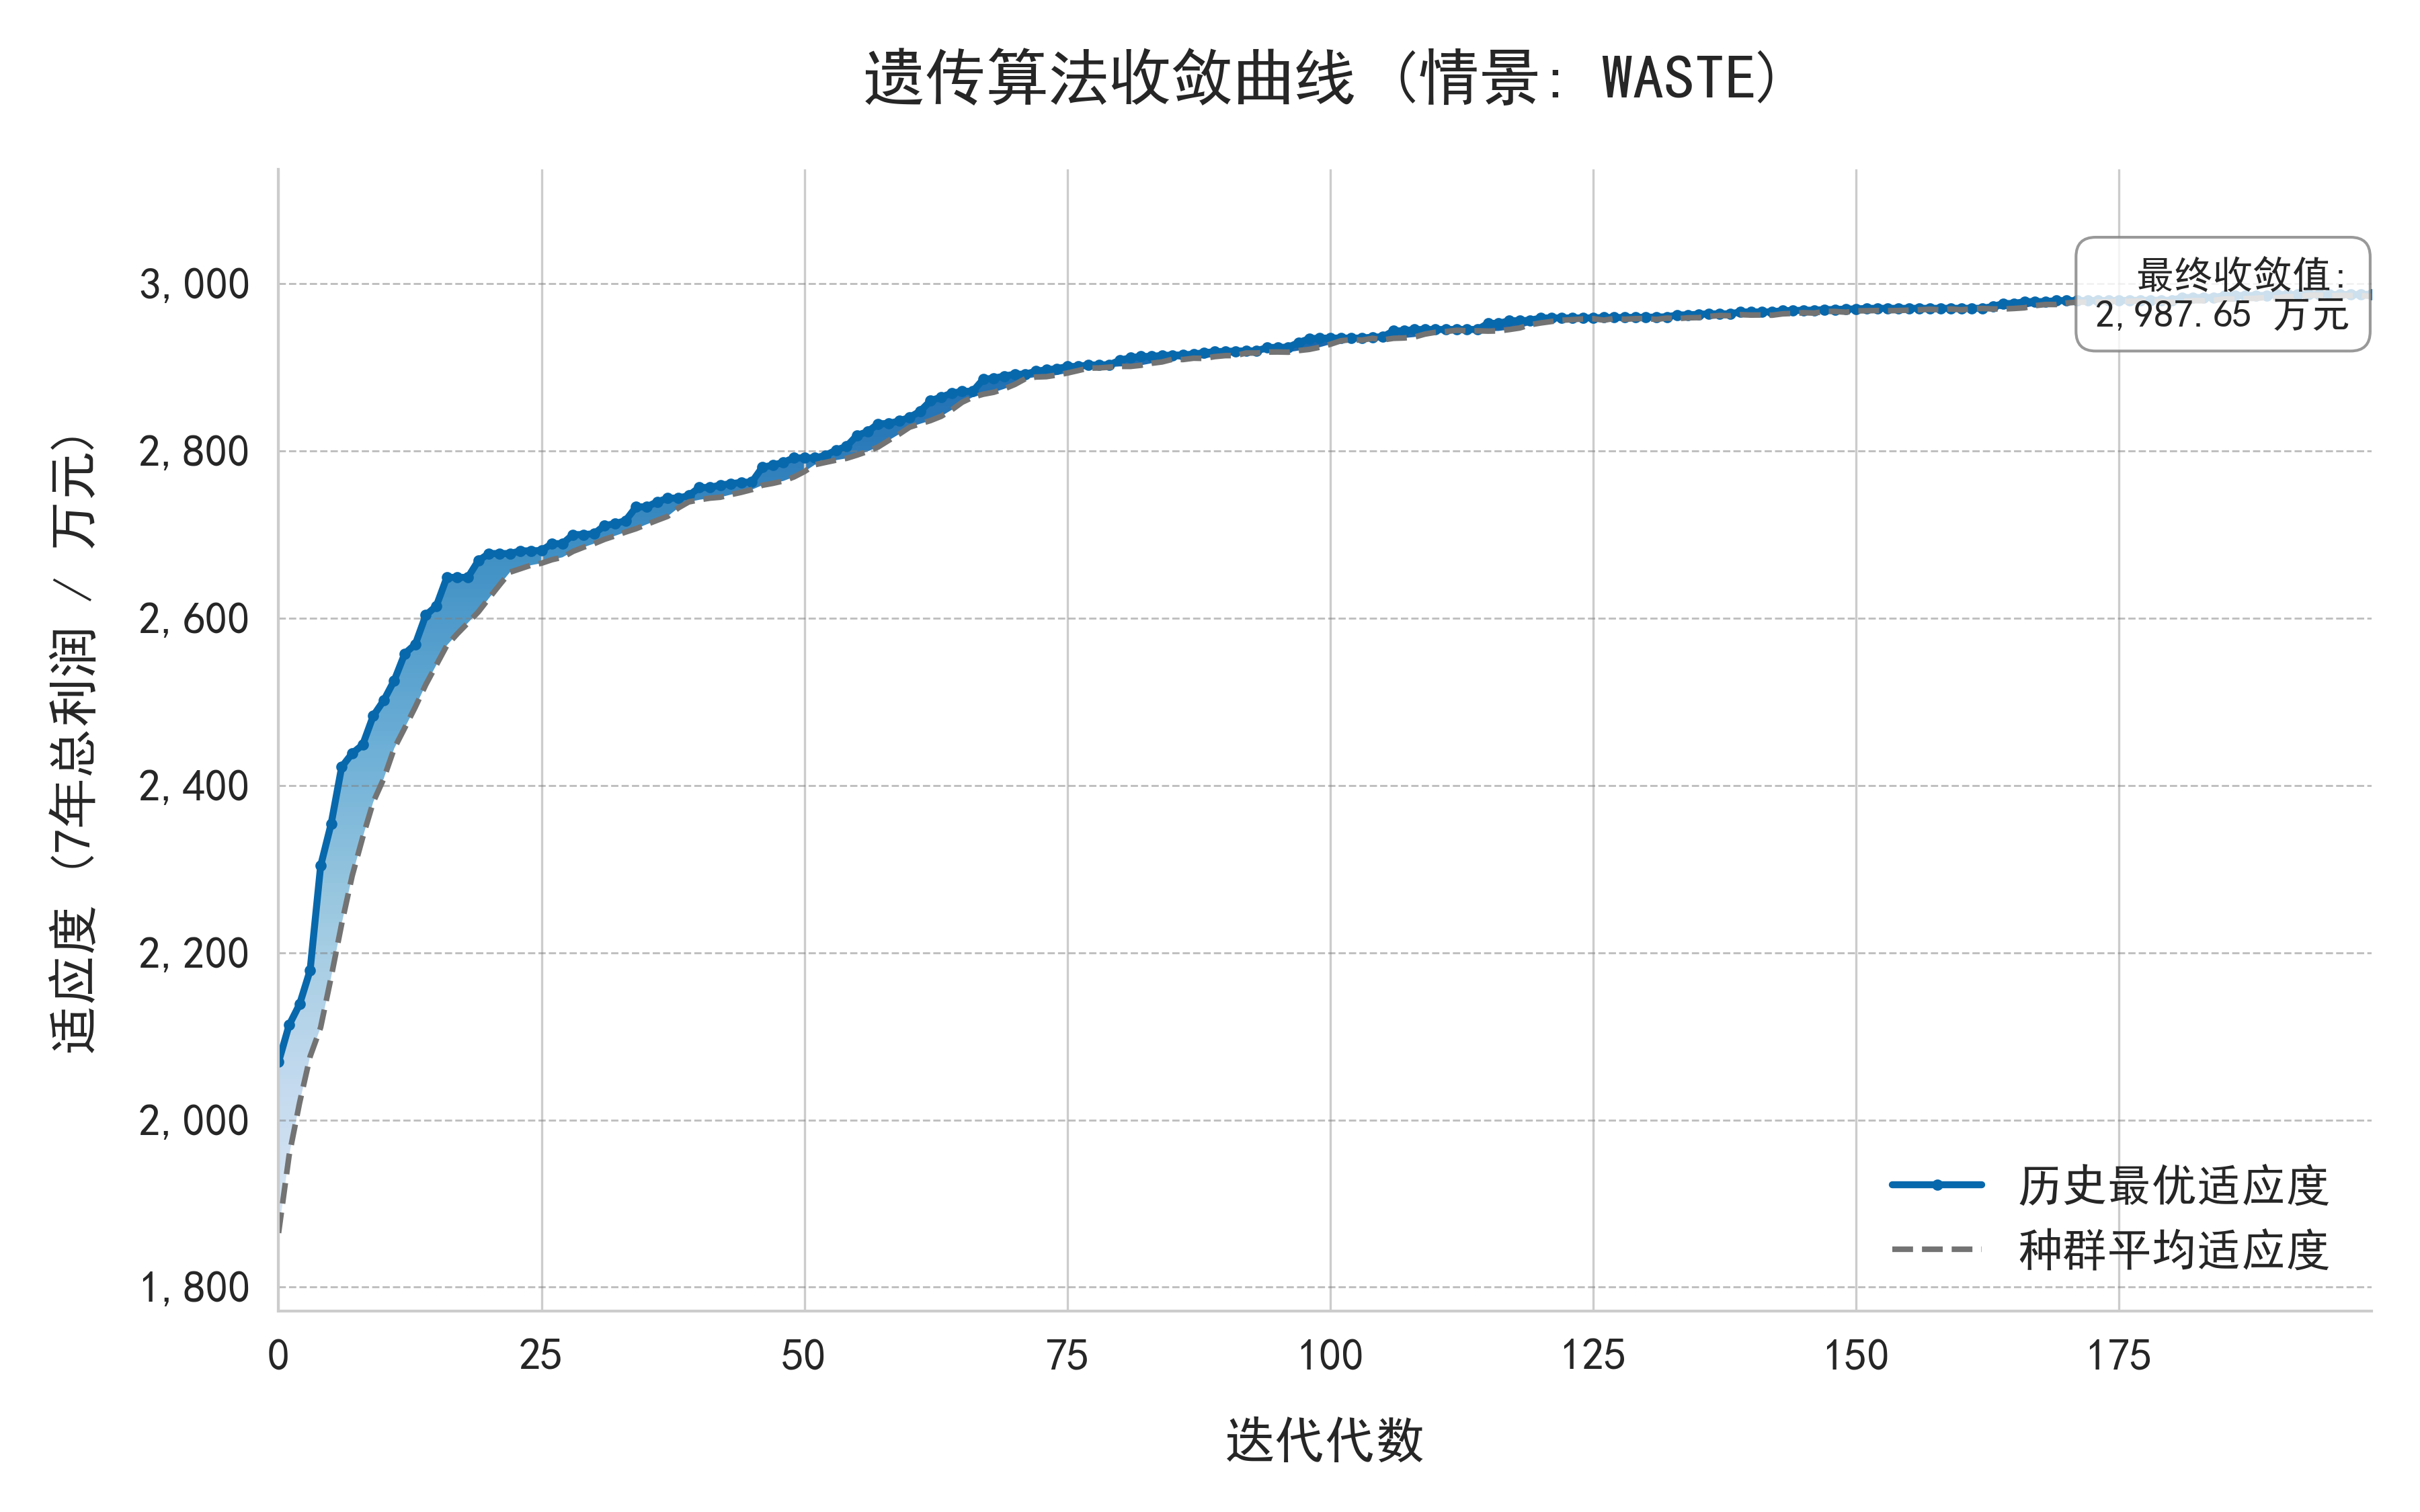
\includegraphics[width=\textwidth]{figs/3问题一/情况一ga训练曲线.png}
        \caption{情景一(超出部分滞销)收敛过程}
        \label{fig:conv_case1}
    \end{subfigure}
    \hfill
    \begin{subfigure}[b]{0.48\textwidth}
        \centering
        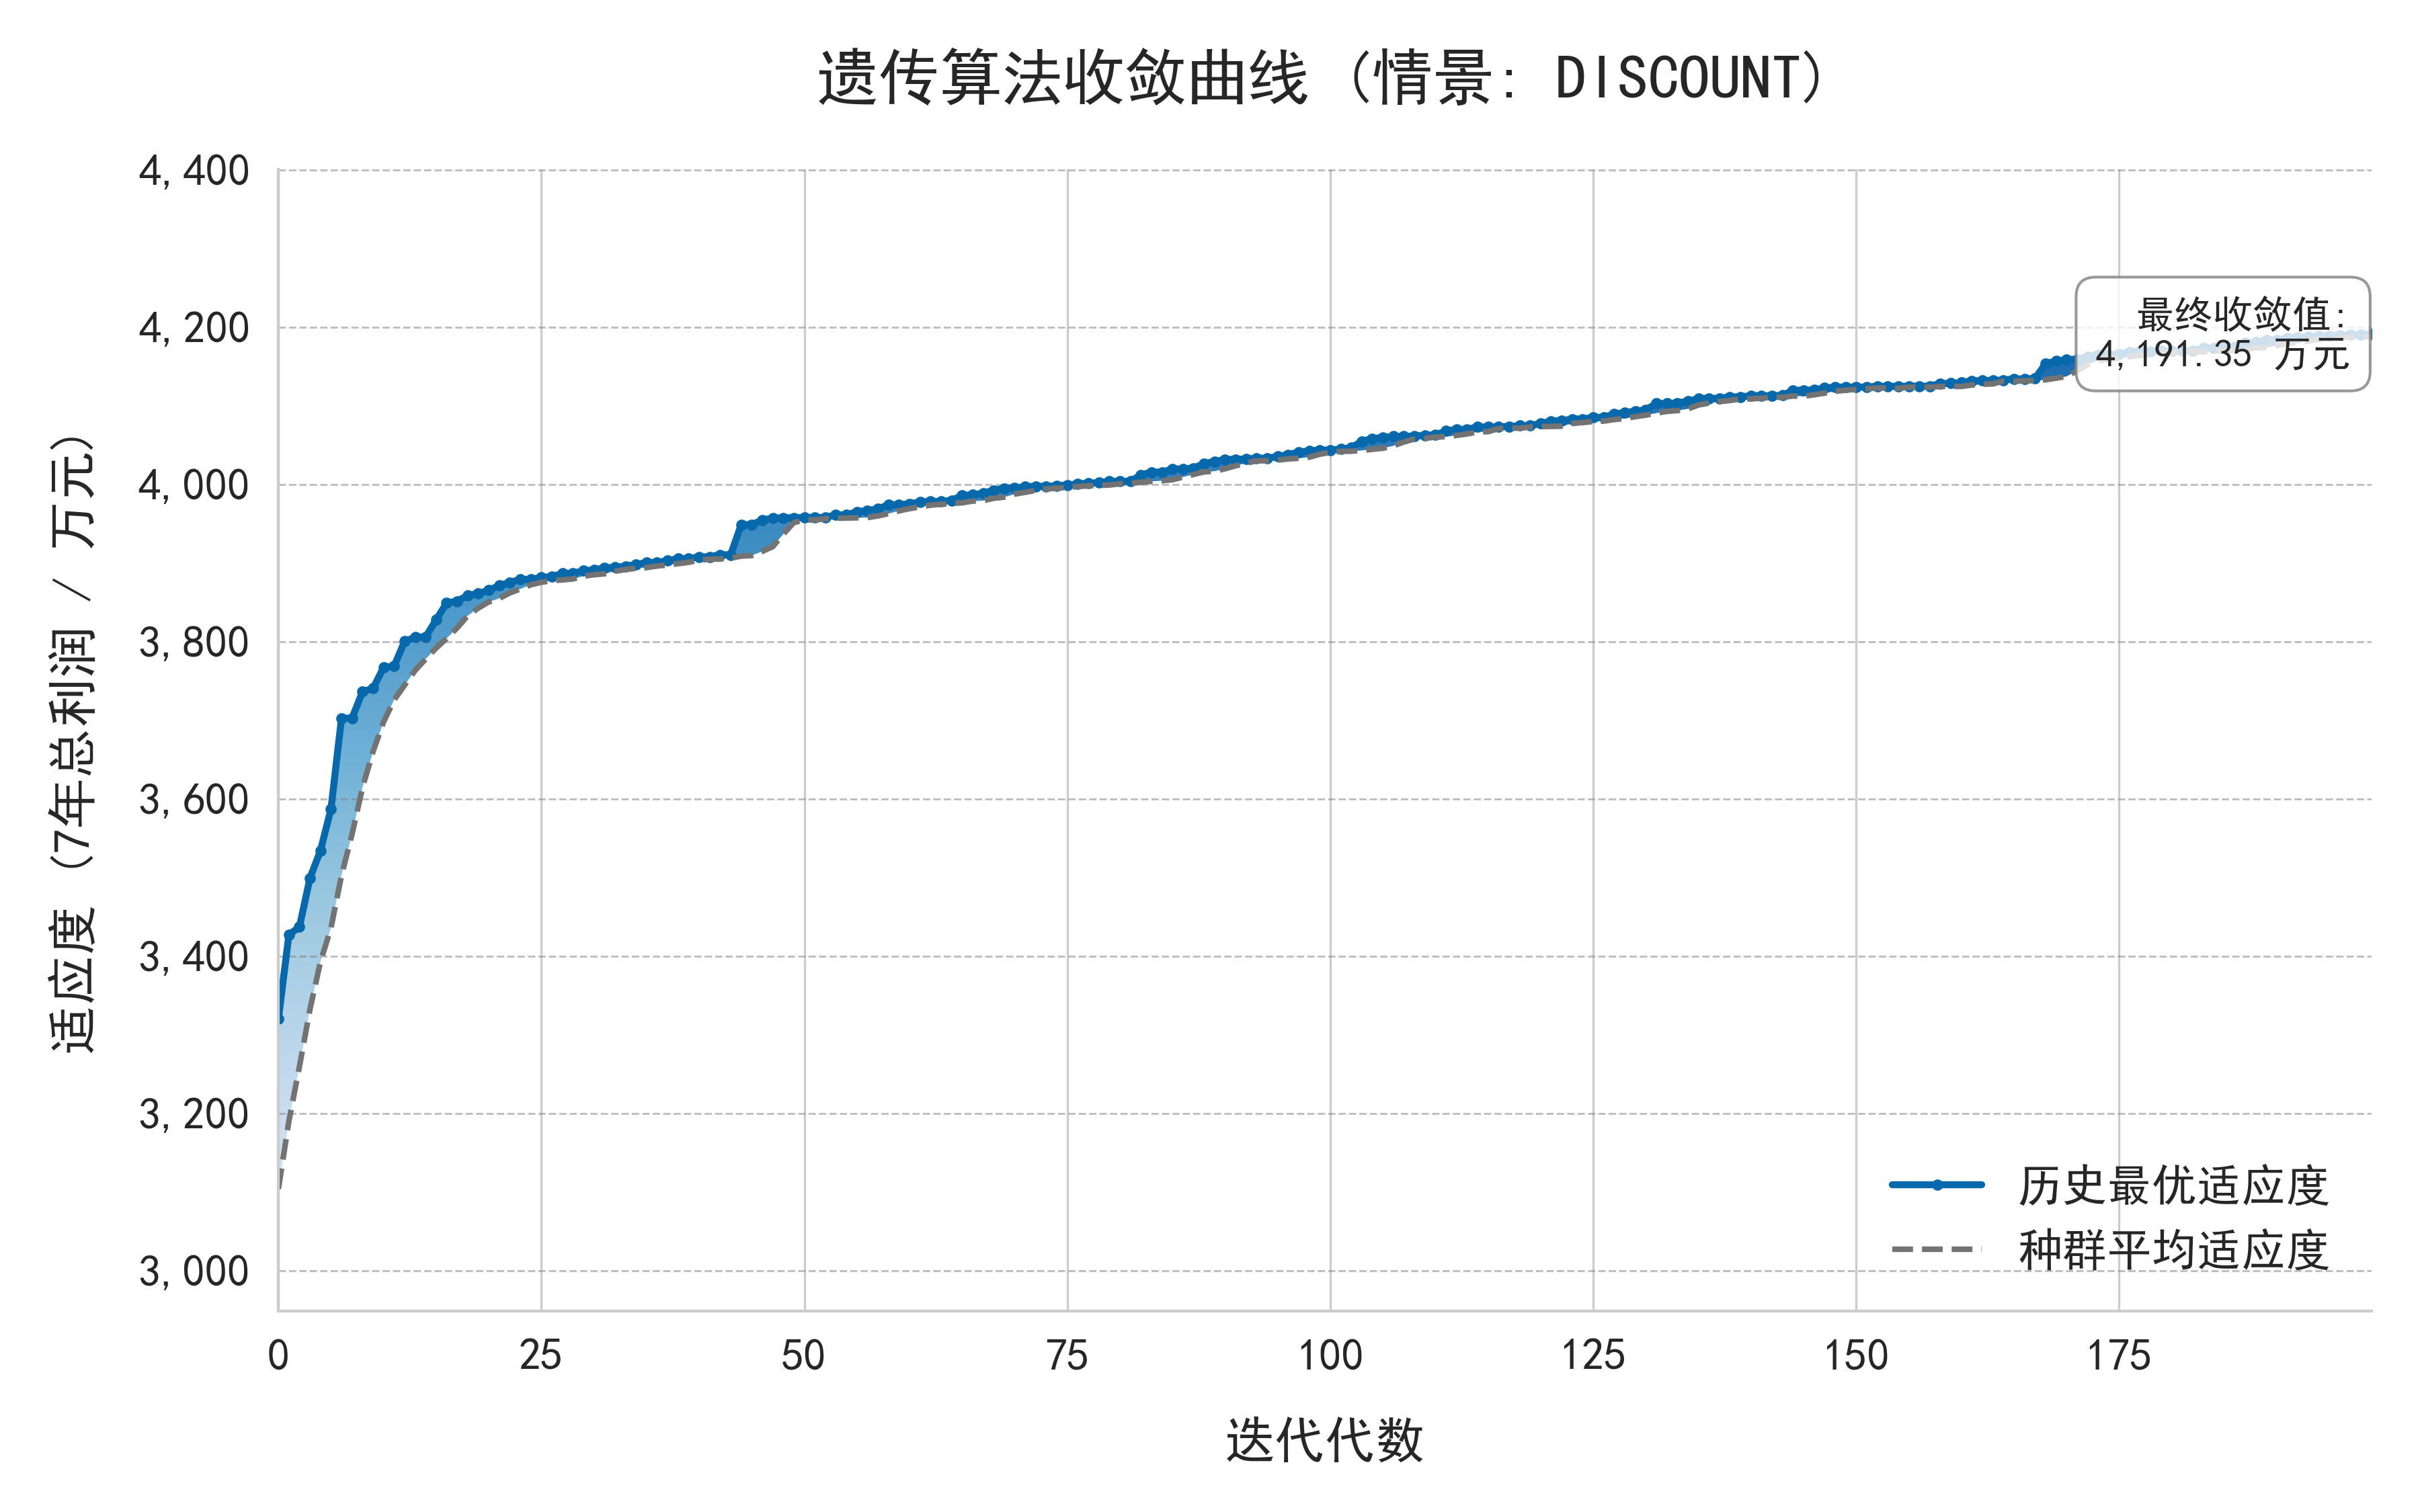
\includegraphics[width=\textwidth]{figs/3问题一/情况二ga训练曲线.png}
        \caption{情景二(超出部分降价)收敛过程}
        \label{fig:conv_case2}
    \end{subfigure}
    \caption{两种情景下修复式遗传算法的适应度收敛曲线。}
    \label{fig:convergence}
\end{figure}

\subsubsection{最优种植方案}
算法求解得到的最优七年种植方案细节繁多,为了直观地展示其时空分布特性,我们采用热力图进行可视化,如图\ref{fig:heatmap}所示。热力图的纵轴代表34个露天耕地地块和20个大棚,横轴为2024至2030年。图中不同颜色对应不同的农作物,清晰地展示了各项作物在不同地块间的轮作模式。

从图中可以观察到,高价值作物(如蔬菜、食用菌)优先被分配到生产效率更高的大棚和水浇地。同时,豆类作物(如大豆)的种植被周期性地安排在各地块中,严格满足了三年至少种植一次的农艺要求。整体方案在空间上呈现出一定的聚集性,有利于规模化管理。

\begin{figure}[H]
    \centering
    \begin{subfigure}[b]{0.45\textwidth}
        \centering
        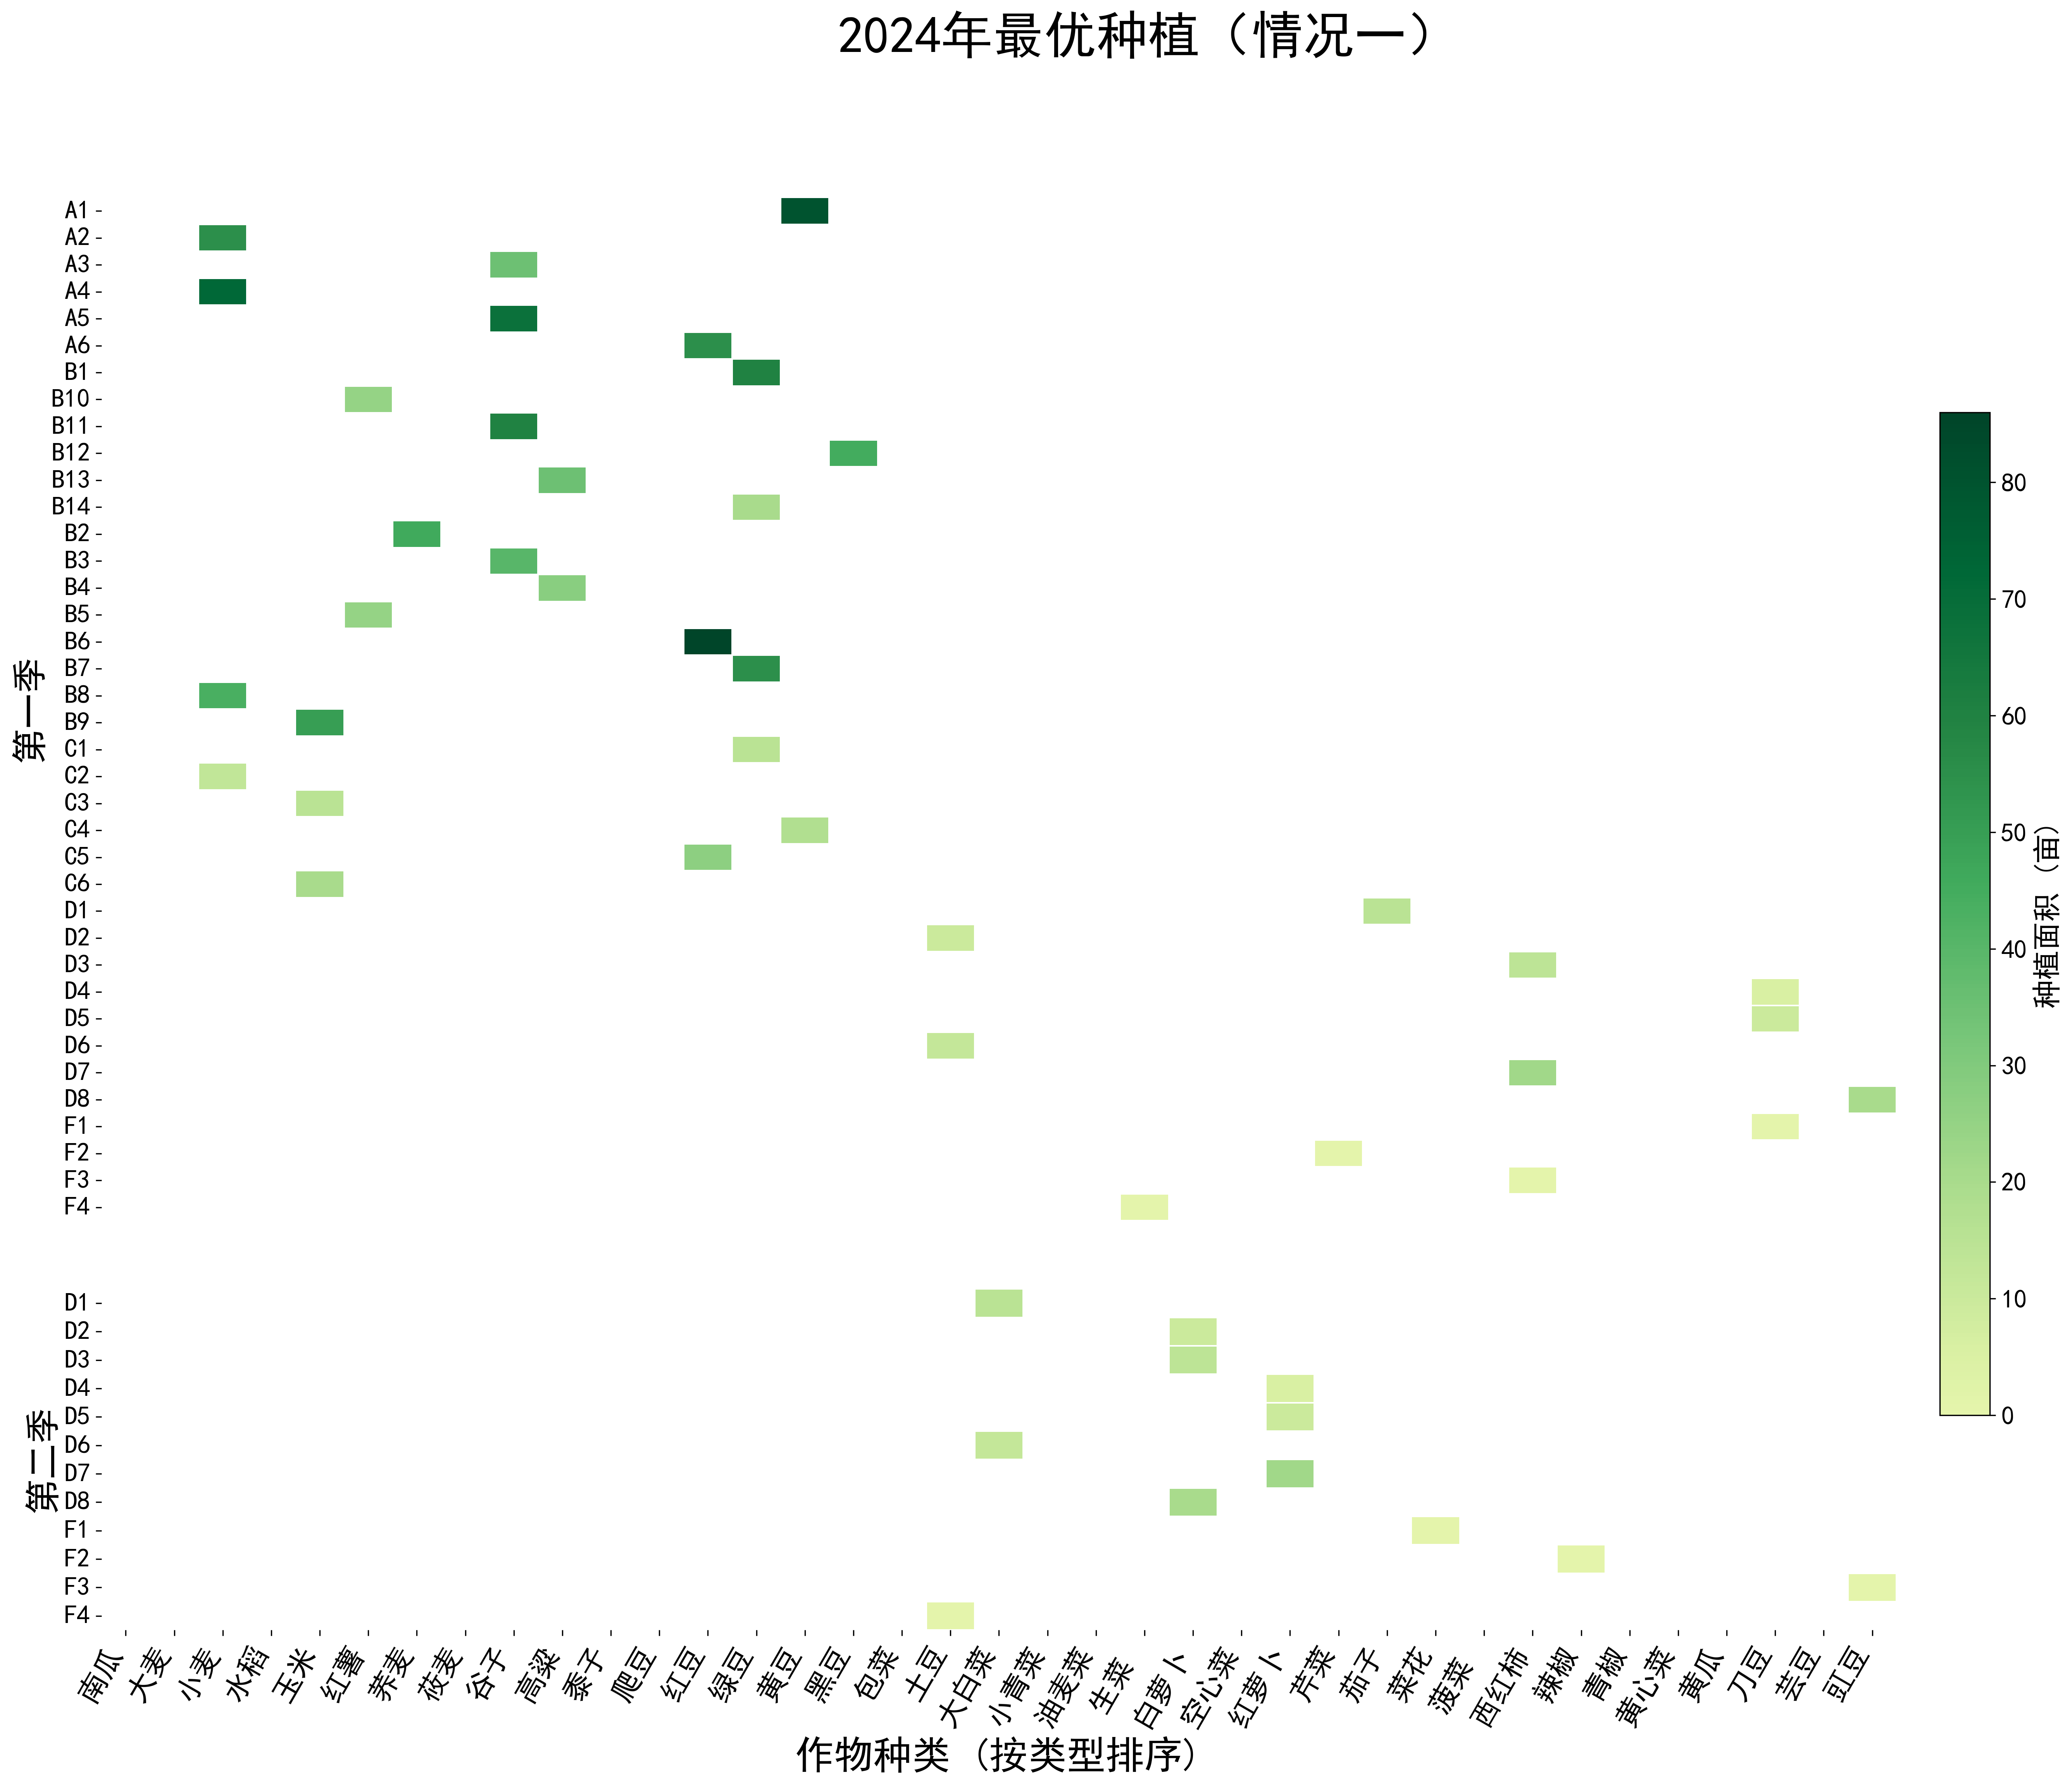
\includegraphics[width=\textwidth]{figs/3问题一/2024年最优种植方案(情况一).png}
        \caption{情景一(超出部分滞销)最优种植方案}
        \label{fig:heatmap_case1}
    \end{subfigure}
    \begin{subfigure}[b]{0.45\textwidth}
        \centering
        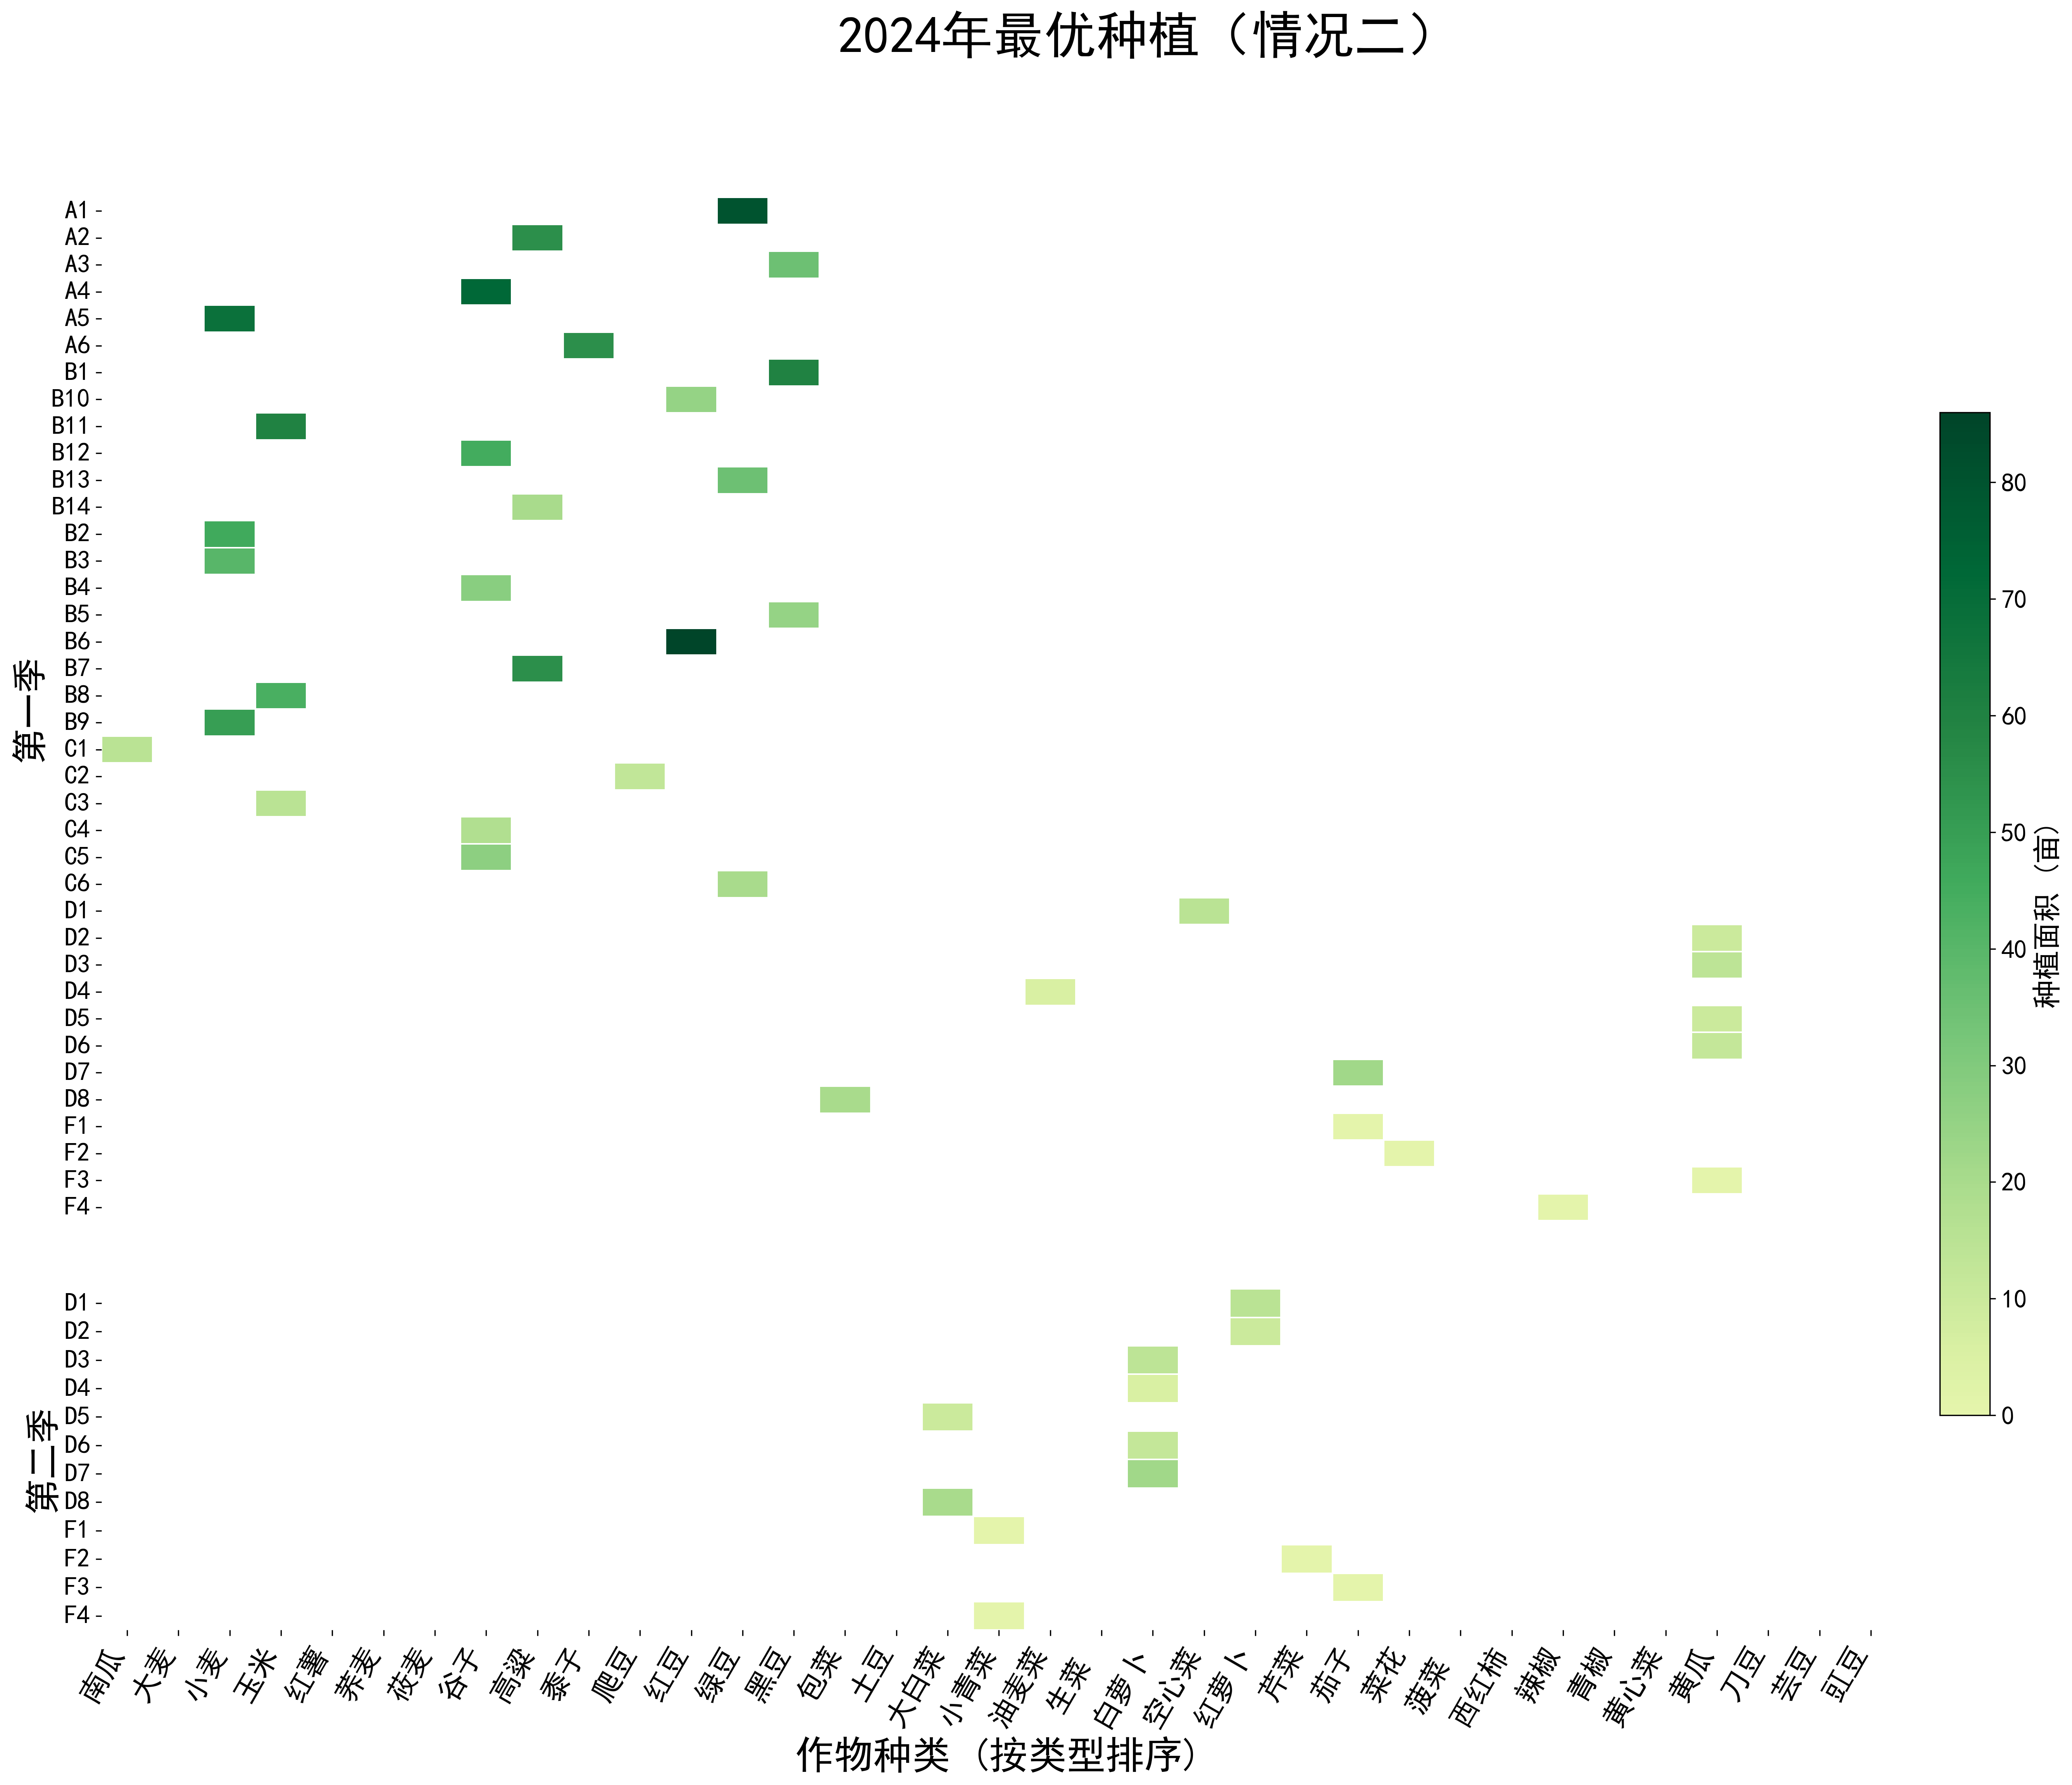
\includegraphics[width=\textwidth]{figs/3问题一/2024年最优种植方案(情况二).png}

        \caption{情景二(超出部分降价)最优种植方案}
        \label{fig:heatmap_case2}
    \end{subfigure}
    \caption{两种情景下2024-2030年最优种植方案时空分布热力图。}
    \label{fig:heatmap}
\end{figure}



